\documentclass{imutthesis}
\chead{\zihao{-5} 云南大学 网络工程}          %页眉内容    
\usepackage{xeCJK} % 声明中文包

\begin{document}
\pagenumbering{gobble}	%无页码
\begin{cnabstract}
    现有传统型高校ICT类专业计算机实验室中,教学流程依赖于教师、学生、实验室器材三个元素,脱离其中任何一个元素实验教学都难以进行。
    
    本次实验针对现有传统型高校ICT类专业计算机实验室的不足进行大胆的改进。具体内容包括结合现有高新技术以及全新概念对实验室提出改造设想和网络系统方案设计两大章。
    
    首先在第一章,当前实验室可以满足一般教学需求,但是在实验设备受限情况下或者现实原因无法在实验室进行的情况下,实验教学就变得难以进行。在此基础上小组成员提出多种已有的高新科技甚至仍在概念中的技术如虚拟现实、元宇宙概念等来设计发展高校ICT类专业计算机实验室。目的使实验室能够实现硬件全仿真、网络资源丰富、操作难度降低等对教学效率有提升的功能。

    其次在第二章,小组成员综合考虑现有高校ICT类专业计算机实验室需求和现实布线、网络结构等因素设计网络系统方案,能够实现网络安全高、流量速度承担的住实际使用。

    通过本次实验,小组成员大胆利用现有技术并结合未来的发展趋势提出元宇宙实验室的构想,最后又趋于现实,结合PT仿真进行ICT类实验室的搭建,在实验过程中,小组成员不仅仅提升了发散性的思维能力,也提高了实验室搭建的动手能力。
    
\par \textbf{关键词}: \textbf{ICT}$\quad$ \textbf{虚拟化}$\quad$ \textbf{元宇宙}    %加粗\textbf{}

\end{cnabstract}

\begin{enabstract}
    In the existing ICT professional computer laboratories of traditional colleges and universities, the teaching process relies on three elements: teachers, students and laboratory equipment, and it is difficult to conduct experimental teaching without any one of them.

This experiment aims at the shortcomings of the existing ICT professional computer laboratories in traditional colleges and universities to make bold improvements. The specific content includes the combination of the existing high and new technology and the new concept of the laboratory to put forward the idea of transformation and network system design two chapters.

First of all, in the first chapter, the current laboratory can meet the general teaching needs, but in the case of limited experimental equipment or practical reasons can not be carried out in the laboratory, experimental teaching becomes difficult to carry out. On this basis, the team members proposed a variety of existing high and new technologies or even technologies still in concept, such as virtual reality, meta-universe concept, to design and develop ICT professional computer laboratories in colleges and universities. Objective To improve the teaching efficiency of the laboratory by full hardware simulation, rich network resources and reduced operation difficulty.

Secondly, in the second chapter, the team members design the network system scheme by comprehensively considering the requirements of ICT professional computer laboratories in colleges and universities, practical wiring, network structure and other factors, so as to realize the practical use of high network security and traffic speed.

Through this experiment, the team members and bold use of existing technology and combined with the future trend of the development of idea of yuan space lab, and finally to the reality, the simulation of PT for the construction of the ICT class laboratory, in the process of experiment, team members not only improved the divergent thinking ability, and improve the ability of laboratory building.

	\par \textbf{Keywords}:  \textbf{ICT}$\quad$ \textbf{virtual}$\quad$ \textbf{Yuan universe}  %加粗\textbf{}

\end{enabstract}

\tableofcontents    %%自动生成目录
\newpage 
\pagenumbering{arabic}
\setcounter{page}{1}
\section{虚拟尽头—元宇宙}
\subsection{发展现状—高校ICT类专业计算机实验室}
\subsubsection{当前高校实验室实现的功能}
随着科学技术的发展,各大高校的ICT实验室的硬件设施已经逐步完善。以云南大学信息学院计算机科学与技术专业各实验室为例,在实验室中,老师可以利用投影与幕布分享桌面,向同学们讲授课堂知识,同时同学们可以利用实验室中的计算机设备进行实验。同时为了避免多人使用设备造成的文件冗杂、系统损坏等情况,目前的ICT实验室的计算机系统已经普遍采用了云桌面技术,在开机后根据预先设置,自动将系统复原。

当前的教学实验室可以满足基础性教学需求与学生的简单实验需求,但实验设备的局限仍然限制着教学的更大范围开展,教学仅限于使用实验室中的硬件设备或虚拟仿真软件。因此,即使高校ICT专业的实验室已经取得了一定的进展,但是能达到的功能还是受到限制,很难紧跟时代和技术的发展,难以给同学们带来优质的实验环境。

\subsubsection{当前高校实验室存在的不足}
\begin{itemize}
    \item \textbf{实验室建设成本问题}
    
    $\qquad$高校ICT实验室建设需要相当高的成本。

    $\qquad$ 第一,为了尽可能满足高校学生的学习需求,高校ICT实验室需要安装足够多的实验设备并保证设备的正常运行。以云南大学信息学院计算机实验室为例,在每个实验室中通常要保证50台以上的计算机设备,多台设备的初始成本已经比较高昂。

    $\qquad$第二,实验室设备维护费用高昂。高校里ICT实验室设备通常需要进行硬件更新与技术更新,以计算机实验室为例,在信息社会发展迅速的今天,计算机技术发展日新月异,高校相关专业的教学大纲也时常更新,一些老旧设备也无法满足当前教学要求,为了尽可能满足学生的实验需求以及时代发展的要求,计算机实验设备需要保持更新状态。同时,由于教学实验室上课学生较多,难以保证学生能够严格按照规定操作设备,导致设备发生损坏,需要进行检修。因此实验室设备的检修与维护也需要较高的费用。
    
    \item \textbf{实验室安全管理上的隐患$^{[1]}$}
    
    $\qquad$ICT实验室是开展科研和教学实验的固定场所,具有危险源多、安全隐患分布广、人员相对集中等特点。在今年11月24日,合肥微尺度物质科学国家研究中心对及时发现并处置实验室漏水的5名学生重奖12万元。据合肥微尺度物质科学国家研究中心发布的通报,由于5名学生的及时得当的处置,避免了至少240万元的财产损失和可能造成的"九章三号"的研发延误。由此可见,实验室的安全管理相当重要,必须常备防水等消防器械,消除实验室中存在的潜在威胁。

    $\qquad$高校教学实验室由于人员较多,尽管多数学校都有实验室安全准入考试,但难以避免学生在实验过程中由于不熟悉实验器材或不清楚实验过程而发生各种各样的意外。像带电拔插接口导致主板击穿从而造成设备损耗这样的细节性意外,难以通过实验室准入考试完全避免。

    \item \textbf{实验室信息化的问题}
    
    $\qquad$当前,高校实验室的信息化管理程度不高,主要表现为实验室管理手段落后,未能有效利用信息化手段实现实验室日常管理、实验室运行数据采集与应用、设备维护与维修及实验物资管理等工作的信息化。

\end{itemize}
\subsubsection{改进方向与提升空间}
实验室虚拟化$^{[2]}$是目前解决以上实验室问题的方法之一,在当前云计算技术、通讯技术、虚拟现实技术的快速发展,实验室虚拟化可以利用强大的云上算力以及极低的传输延迟,实现实验室设备的虚拟、实验过程的虚拟、实验流程的虚拟.....实验室虚拟化有力地解决了实验室硬件设备成本高昂、管理复杂、信息化程度低的问题,同时,只需要对虚拟系统进行软件更新即可实现实验设备的更新。

在以往的教育中,学习者始终生活在两个世界的时空环境中,一个是经验世界(实践中学习),另一个是语言文字的世界(书本中学习),两者往往相互脱节,即理论脱离实际。而由多媒体与仿真技术相结合产生的虚拟现实技术,创造出了第三个世界-----虚拟现实世界,它将成为沟通前两个世界的重要桥梁。我把“三个世界”的学习经验综合起来,促成三者的有机结合。要充分利用虚拟现实情境之独特优势,去引导和促进学习者在经验世界和语言文字世界中实现学习活动与学习经验的整合,不断激励和提高学习者在“三个世界”中学习的自主性、协作性和创造性。

\subsection{前沿技术—虚拟现实实验室}
\subsubsection{前沿技术介绍}
\begin{itemize}
    \item \textbf{图像识别技术(Image Recognition Technology
    )}
  
    $\qquad$图像识别技术是对图像进行对象识别,以识别各种不同模式的目标和对象的技术。

    $\qquad$为了编制模拟人类图像识别活动的计算机程序,人们提出了不同的图像识别模型。例如模板匹配模型。这种模型认为识别某个图像,必须在过去的经验中有这个图像的记忆模式,才能进行图像识别。这个模式识别的模板匹配模型简单明了,也容易得到实际应用。但是这种模型强调图像必须与模板完全符合才能加以识别。

    \item \textbf{虚拟现实技术(Virtual Reality, VR
    )}

    $\qquad$虚拟现实技术是20世纪发展起来的一项全新的实用技术。可以让用户沉浸于由计算机生成的三维虚拟环境,并与现实环境相隔绝。其基本实现方式是计算机模拟虚拟环境从而给人以环境沉浸感。

    \item \textbf{增强现实技术(Augmented Reality, AR
    )}

    $\qquad$增强现实技术是在真实环境中增添或者移除由计算机实时生成的可以交互的虚拟物体或信息。

    \item \textbf{动作捕捉技术(Motion capture
    )$^{[3]}$}

    $\qquad$动作捕捉技术是通过在运动物体的关键部位设置跟踪器,由Motion capture系统捕捉跟踪器位置,再经过计算机处理后得到三维空间坐标的数据。数据被计算机识别后,录入系统,应用在动画制作,步态分析,生物力学,人机工程等领域。

\end{itemize}
\subsubsection{前沿技术应用}

图像识别技术是立体视觉、运动分析、数据融合等实用技术的基础,在众多领域有重要的应用价值。如:遥感图像识别:航空遥感和卫星遥感图像通常用图像识别技术进行加工以便提取有用的信息;通讯领域的应用:包括图像传输、电视电话、电视会议等。

虚拟现实技术已经部分应用在了理工专业,如Solidworks与Unity 3D联合设计开发的3D铸造仿真实训系统 和电力系统现实仿真系统 ,云南大学也曾设计出一个物联网装置的虚拟仿真项目。

增强现实技术也在逐渐普及,无论是全球收集“宝可梦”的游戏设计还是历史遗迹保护重现的现代技术,都在促进着AR技术的发展和提高。

虚拟现实与增强现实技术交叉使用在教育教学中的应用也最为广泛。在麻醉学教学 中的应用,涵盖了麻醉学技能培训、情景模拟教学、危机管理培训、医患沟通与远程教学等各个方面,在教育实践与培训中展现出广阔的应用前景。这也为我们利用AR和VR技术来进行实验室的教学改革建设提供借鉴与参考。

美国海军在测试哥伦比亚大学开发的现实增强软件,用来在机械维修领域的教学工作。他们用了一个头盔,可以将计算机生成的3D图像覆盖在需要维修的设备之上,将每个部件标上名称,然后给出一步一步的指导。
\begin{figure}[htbp]
    \centering
    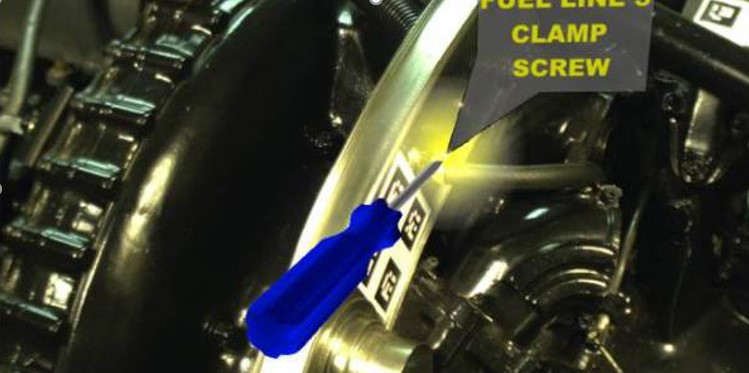
\includegraphics{现实.jpg}
    \caption{现实增强技术的实例}
\end{figure}
\newpage
西雅图大学研究生物神经科技的Parviz副教授制作了一个隐形眼镜,含有一个微小、透明的电路板,电路板里有一个LED,这个镜片会接收身边智能手机传出的无线信号,现在已经成功实现了声文转换。在未来的几年里,他想要在镜面上增加上百的LED,这将使文字和图片飘浮在眼睛可以读取的距离之内。它以后甚至可以将你说的话直接转换为文字,成为聋哑人的有力助手。

\subsubsection{改进教学条件提供的优势}
在以往的教育中,学习者始终生活在两个世界的时空环境中,一个是经验世界(实践中学习),另一个是语言文字的世界(书本中学习),两者往往相互脱节,即理论脱离实际。而由多媒体与仿真技术相结合产生的虚拟现实技术,创造出了第三个世界-----虚拟现实世界,它将成为沟通前两个世界的重要桥梁。把“三个世界”的学习经验综合起来,促成三者的有机结合。要充分利用虚拟现实情境之独特优势,去引导和促进学习者在经验世界和语言文字世界中实现学习活动与学习经验的整合,不断激励和提高学习者在“三个世界”中学习的自主性、协作性和创造性。

拓宽视野,激发学习热情。
通过虚拟现实技术,一方面可以再现实际生活中无法观察到的自然现象或事物的变化过程,为学习者提供生动、逼真的感性学习材料,使抽象的概念理论直观化、形象化,方便学习者对抽象概念的理解;另一方面虚拟现实技术使学习者能够按自己的需要来进行实时的交互式学习,主动地获取所需要的知识,由被动式的接受转化为主动式的发现。

\begin{figure}[htbp]
    \centering
    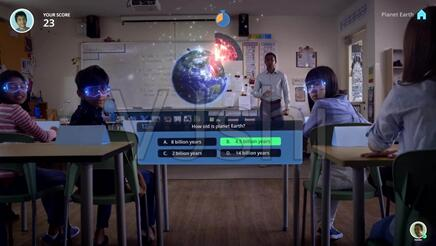
\includegraphics{第三世界.jpg}
    \caption{虚拟教学概念图}
\end{figure}
\begin{itemize}
    \item \textbf{提高学生动手能力}
    $\qquad$学生群体普遍存在理论能力良好而实践能力较差的问题,如果实验室硬件设备数量不足甚至设备缺乏,更会导致学生动手能力差上加差。而利用VR、AR等新技术搭建的实验室,可以完美解决设施无法匹配学生的需求这一问题,可以让学生人均一台设备进行操作,增加实践机会,提高动手能力。
    \begin{figure}[htbp]
        \centering
        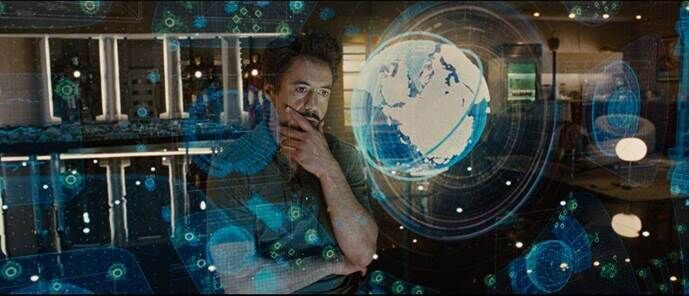
\includegraphics{托尼.jpg}
        \caption{提高学生动手能力}
    \end{figure}
    \item \textbf{降低教学成本}
    
    $\qquad$高校实验室普遍存在教学经费紧张的问题,故而出现设备损耗时往往难以立刻维修或者更新。而学生群体由于缺乏经验,经常出现误操作导致设备损耗的问题。利用虚拟实验室可以有效避免出现设备损耗的情况。通过设置一定的惩罚机制,既可以让学生体会到操作错误的后果,又能节约资金,降低教学成本,提高教学效果。
    \item \textbf{促进教育公平}
    
    $\qquad$由于不同地域的经济水平差异,学校用于学生动手实训的经费也各有不同,实验室的配置也相差万千。经济发达地区的学校相对经济水平一般地区的学校,经济水平高,教学经费充足,设备状况优良。这就直接影响了教育公平在高等教育阶段的开展与落实。通过在实验室中利用虚拟现实、增强现实技术等诸多新型技术的进行教学,将价格高昂的设备变成虚拟的数据,将虚拟的数据转化为学生可以感知可以去体验的设备,让更多的学生群体能够亲身去体会,去学习更多的动手操作,无疑是促进教育公平、提高学生群体的水平的一大重要举措。 
    \item \textbf{提高教学效果}
    
    $\qquad$在拥有物理基础的实验室中,可以通过部署图像识别技术,将动作识别、机器识别等加入到虚拟实验室中。通过捕捉动作实现3D投影等技术的人机实时交互,使得教学更加仿真,更加传神,并且可以实现实验室内围观操作放大直接上手操作、实验室外的大型施工缩小直接模块化操作等。
    \begin{figure}[htbp]
        \centering
        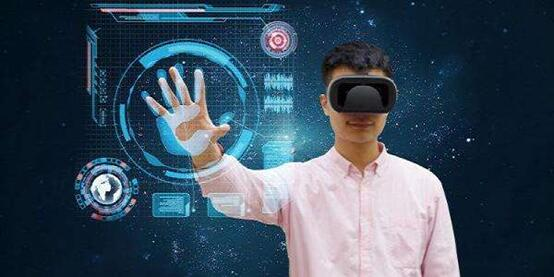
\includegraphics{提高.jpg}
        \caption{提高教学效果}
    \end{figure}

\end{itemize}
\subsection{未来趋势—元宇宙实验室}
\subsubsection{元宇宙$^{[4]}$的概念}
元宇宙(Metaverse)是利用科技手段进行链接与创造的,与现实世界映射与交互的虚拟世界,具备新型社会体系的数字生活空间。
它整合了多种新技术而产生的新型虚实相融的互联网应用和社会形态,它基于扩展现实技术提供沉浸式体验,基于数字孪生技术生成现实世界的镜像,基于区块链技术搭建经济体系,将虚拟世界与现实世界在经济系统、社交系统、身份系统上密切融合,并且允许每个用户进行内容生产和世界编辑。

元宇宙本质上是对现实世界的虚拟化、数字化过程,需要对内容生产、经济系统、用户体验以及实体世界内容等进行大量改造。但元宇宙的发展是循序渐进的,是在共享的基础设施、标准及协议的支撑下,由众多工具、平台不断融合、进化而最终成形。

\subsubsection{元宇宙实验室的构想}
利用元宇宙技术,以数字化信息为基础,对学校的教学、科研、管理和生活服务等所有信息资源进行全面的数字化,最终实现教育的信息化,提高学校的办学水平和管理水平。
元宇宙实验室主要从事虚拟现实技术、可视化技术、计算机网络、图形系统工具、图像信息处理、分布式系统和人工智能等领域的科学研究和技术开发。

发挥学校学科专业优势,积极利用企业的开发实力和支持服务能力,充分整合学校信息化实验教学资源,以培养学生综合设计和创新能力为出发点,创造性地建设与应用高水平软件共享虚拟实验、仪器共享虚拟实验和远程控制虚拟实验等教学资源,提高教学能力,拓展实践领域,丰富教学内容,降低成本和风险,开展绿色实验教学。

\subsubsection{元宇宙实验室的建设}
为了更好的应用虚拟现实技术,使其更好的应用于教学、科研和生产实践活动,推出全面的元宇宙实验室整体系统建设方案。以下方案供参考:
\begin{itemize}
    \item \textbf{虚拟现实应用开发引擎}
    
    (1)Unity3D PRO 虚拟现实、跨平台应用程序开发引擎

    $\qquad$Unity3D是一软专业3D游戏引擎,其备跨平台发布、离效能优化、高性价比,AAA级游戏画面演染效果等特点。目前Unity3D应用范围广泛,从手机游戏到联网的大型游戏,从严肃游戏到电子商务,再到虚拟现实VR均可完美呈现。

    (2)MiddleVR for Unity插件

    $\qquad$Unity为一款3D应用程序开发工具,设计为使您能够专注于创造令人惊叹的3D应用。”Middle VR是一个完美的插件,可在几分钟内为你的Unity应用程序带来身临其境的性能!Middle VR为Unity增加了以下功能:提升了以用户为中心视角的可视化级别 、支持3D交互设备,如3D跟踪器、S3D - 主动,被动...、适用于更高分辨率和令人印象深刻的VR系统的多屏幕/多台计算机同步。
    \item \textbf{沉浸式环境-单通道投影}
    
    $\qquad$立体投影系统有被动式立体投影和主动式立体投影,被动式立体投影是通过光的偏振原理来实现的,即采用两台投影机同步放映图像,将两台投影机前的偏光片的偏振方向互相垂直,让产生的两束偏振光的偏振方向也互相垂直。而偏振光投射到专用的投影幕上再反射到观众位置时偏振光方向须不改变,观众通过偏光眼镜每只眼睛只能看到相应的偏振光图像,从而在视觉神经系统中产生立体感觉;主动式立体投影需要内置液晶(LCD)快门的眼镜来交替地空白左右眼信息。一个分离的IR发送器发送同步信息到眼镜。这种方法在技术上更耐用,且投影机必须配备空白间隔的与快门速度相匹配。主动式立体投影的优点是可在任何投影屏幕上来实现。

    \item \textbf{VR交互系统 (5DT数据手套、ART光学定位追踪系统)}
    
    (1)5DT Data Glove 14 Ultra数据手套:1只

    $\qquad$5DT Data Glove 14 Ultra可测量手指弯曲的程度与手指间的外部肌肉(每只手指上有2个传感器),是5DT公司为现代动作捕捉和动画制作领域的专业人士专门设计的一款数据手套产品,可满足最为苛刻的工作要求。该产品具有佩戴舒适、简单易用、波形系数小、以及驱动程序完备等特点。超高的数据质量、较低的交叉关联、以及高数据频率使该产品成为制作逼真实时动画的理想工具。

    (2)A.R.T smARTtrack 光学跟踪系统

    $\qquad$smARTtrack是一款全集成独立红外光学跟踪系统,专门用于小空间内(约2立方米)的目标跟踪。典型的应用领域包括: 工作台上的工程或设计审查 、使用立体电视或者头盔显示器进行的员工培训 、在上述应用中,该产品是头部跟踪或者与互动装置配合使用的理想产品。在有源立体应用当中,可以安装外部同步系统。smARTtrack经过预先校准,所以使用前不必进行校准。

    (3)A.R.T.Flystick2 交互设备

    $\qquad$Flystick2是一款用于虚拟现实应用领域的无线式交互设备,是以往Flystick的更新产品。该产品升级为6个按钮并配有模拟操纵杆。DTrack软件用于控制Flystick2按钮和操纵杆,并使用6自由度输出数据使其相互关联,从而使得全部数据的匹配过程变得简便而轻松。

\end{itemize}

\subsubsection{元宇宙实验室的优点}
具体来说,利用沉浸式虚拟实验室进行实验教学具有以下价值:

(1)减少实验室建设的资金和空间投入、弥补实验场地的不足;

(2)节省实验器材的损耗,缓解设备的缺少或陈旧带来的压力等情况;

(3)避免实验中的危险和危害,降低污染;

(4)更新教学观念,教师由知识讲授的权威者、讲授者转变为实验的设计者、引导者和组织者,学生由知识容器和知识受体转变为学习主体,主动获取知识;

(5)提供实时监测、模拟自检等多种训练模式,给予反馈性提示;

(6)促进开放式、个性化教学。沉浸式虚拟实验室通过三维模型和训练环节能够有效集中学生注意力、吸引学生学习兴趣、提高学生动手能力,促进学生转变“学习只能依靠被动接受”的固化思维,主动学习和模拟训练,可以不受传统实验室开放时间的限制,灵活安排自己的实验时间,也可以根据自己的进度或兴趣选择实验内容进行课外拓展和补充;

(7)引导横向拓展与纵向应用相结合。沉浸式虚拟实验室的横向拓展是指由教学者开发设计性和综合性实验,提高学生实验动手能力,增强科学实验素养;纵向应用是指开设新技术成果的应用以及其他新型实验,提供相应的实验课题,由学习者根据个人兴趣和能力选择进行实验探究,培养学生的创新能力等。对于实验这种需要学习者亲身参与的实践活动来说,沉浸式虚拟实验室是一种发展趋势,更是一种创新变革的教学应用。
\subsubsection{元宇宙教学应用}
其实元宇宙在教育领域的应用疫情之下已有显现,全球顶级AI学术会议之一的ACAI,把2020年的研讨会放在了任天堂的《动物森友会》上举行;中国传媒大学为了不让学生因为疫情错过毕业典礼,在沙盘游戏《我的世界》里重建了校园,学生化身成为游戏人物形象齐聚一堂完成仪式。

“元宇宙特别适合运用于沉浸式学习,它给学生创造了更身临其境的学习空间。”,利用元宇宙对计算机的原理进行仿真,将自己想象成一个数据,去研究计算机组成原理、去学习计算机网络的报文协议、去实现交换机、路由器的真实配置……利用元宇宙,知识不再是抽象枯燥的,将会变成真正现实可感知的。

元宇宙的另一重要作用是节约教育成本。在科研教育中,元宇宙技术可以模拟出昂贵的教学设备,还原机械设备的同时,还能够辅助教师进行教学。元宇宙技术可以大大节约教育成本。应用到强电流环境下的实验操作、昂贵设备的模拟、机器人零部件的配置等领域,这极大程度上降低实验损耗,在高危险系数的实验中更能起到保护师生生命安全的作用。

此外,元宇宙中的“理想课堂”还会提升课堂效率和学生学习兴趣。教师可以根据自己的喜好,设置设定自己喜欢的任何形象,授课教师也可能是司马迁或者爱因斯坦。每个反应可以变成一个具象化的符号,比如某个学生对教师的讲解表示疑惑,头上就会蹦出一个问号,方便教师及时捕捉反馈。”


\section{网络系统方案设计}
\subsection{需求分析}
高校 ICT 类专业计算机实验室在云技术的基础上承担学生日常上机实验课,教师为学生提供教学演示、控制、投屏到学生机等任务。
\subsubsection{功能需求$^{[5]}$}
(1) ICT 类实验室网络具有高速、大流量并发的特点,且需要支持稳定、快速高效的传输文件或视频、声音等流媒体的功能,二级以上的交换机应具备组播功能。

(2) ICT 类实验室应具备性能优越的资源共享功能,使计算机资源得到高效利用,让学生能够高效接收老师分享的文件或展示的共享屏幕等。

(3) ICT 类实验室应具备高效的管理效率,让教师对同学们的实验设备具有高效的控制和管理,方便教师维护教学秩序。

(4) ICT 类实验室应方便维护和管理,软件更新方便快捷,减少同学们在维护设备等方面消耗的精力,让同学们可以专心于实验。

(5) ICT 类实验室内学习不受时间和空间制约,学生只需要在计算机上登录客户端搜索相关知识即可自学。

(6) ICT 类实验室系统运行节点故障后,学生的学习操作不受故障影响,终端不会停止。 
\subsubsection{设计原则}
(1)经济实用性
遵循经济实用的原则。采用云架构可循环利用淘汰计算机,作为云计算的终端机利用,这样就可以降低计算机实验室的投建成本,大大提升陈旧计算机的使用率,提高其服务质量和水平。

(2)可靠性
为保证 ICT 类实验室可靠稳定运行,从网络结构、技术措施、设备性能、系统管理等方面提供优先保障,在遇到问题时有配套的技术措施作为后备保障。

(3)可升级和可扩展性
选择具有扩展余量的网络设备,在分配 IP 时也要留有余量,方便后续添加终端或升级网络设备。

(4)容错性
设备容错性:所选用设备必须具有全容错结构,一台设备中单个电源、单个风扇的故障不影响设备工作,单个模块的故障不影响其它模块的正常工作。

网络结构容错:不能因某台设备的故障而影响到整个主干网络的正常运行;任意一条链路的中断不能使得主干网络的任何部分中断工作。


\subsection{系统主要节点流量分析}
经过实际考察,结合实验室的需求,估算出以下公式:应用总信息传输速率 平均事务大小 × 每字节位数 × 每个会话事务数 × 平均用户数/平均会话长度

在 ICT 类实验室中,根据实际需求,实验室中实际使用的流量在300~500Mbps,此处我们假设为 500Mbps。我们使用的四台交换机是S5730-60C-HI。

需求分析表:
\begin{table}[h]%htbp表示的意思是latex会尽量满足排在前面的浮动格式,就是h-t-b-p这个顺序,让排版的效果尽量好。
    \centering
    \begin{tabular}{p{2.0cm}<{\centering}p{9.0cm}<{\centering}p{2.0cm}<{\centering}}
 %指定单元格宽度, 并且水平居中。
    \hline
    需求事务 & &所需流量  \\ %换行 
    \hline
    在线学习 & & 50Mbps \\ 
    文件共享 & & 150Mbps \\ 
    视频监控 & & 100Mbps\\
    下载服务 & & 100Mbps\\
    教学游戏 & & 50Mbps\\
    其他 & & 50Mbps\\
    \hline
    \end{tabular}
\end{table}

节点流量分析:
\begin{table}[h]%htbp表示的意思是latex会尽量满足排在前面的浮动格式,就是h-t-b-p这个顺序,让排版的效果尽量好。
    \centering
    \begin{tabular}{p{5.0cm}<{\centering}p{9.0cm}<{\centering}p{2.0cm}<{\centering}}
 %指定单元格宽度, 并且水平居中。
    \hline
    节点 & 流量  \\ %换行 
    \hline
    核心交换机  &  1000Mbps(实际中使用假设500Mbps) \\ 
    工作交换机 &  100Mbps \\ 
    PC机(PC01-PC25) &  25台PC机共享100Mbps(平均每台4Mbps)\\
    PC机(PC26-PC50) &  25台PC机共享100Mbps(平均每台4Mbps)\\
    PC机(PC51-PC75) &  25台PC机共享100Mbps(平均每台4Mbps)\\
    PC机(PC76-PC100)&  25台PC机共享100Mbps(平均每台4Mbps)\\
    \hline
    \end{tabular}
\end{table}

\subsection{网络拓扑图设计}
\begin{figure}[htbp]
    \centering
    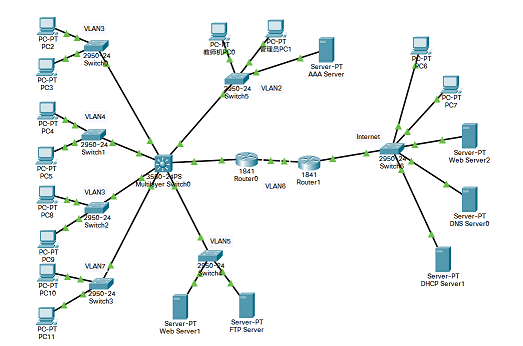
\includegraphics{网络拓扑图.png}
    \caption{网络拓扑图}
\end{figure}

由计算可以知道,若需要将100台PC机之间实现通信的话,会用到5台两层交换机(每台双层交换机有24个口),实验中为了简单起见每台交换机只连接两台计算机,在这里我们还要实现不同VLAN下PC机之间的通信所以还需要借助一台三层交换机。

\subsection{PT模拟仿真}

IP地址规划:
\begin{table}[h]%htbp表示的意思是latex会尽量满足排在前面的浮动格式,就是h-t-b-p这个顺序,让排版的效果尽量好。
    \centering
    \begin{tabular}{p{2.6cm}<{\centering}p{4.4cm}<{\centering}p{3.0cm}<{\centering}p{2.0cm}<{\centering}p{2.0cm}<{\centering}p{2.0cm}}
 %指定单元格宽度, 并且水平居中。
    \hline
    设备 & IP地址 & 子网掩码 & 默认网关 & VLAN & 交换机  \\ %换行 
    \hline
    PC0-PC25  & 192.168.2.1-192.168.2.25 & 255.255.255.0 & 192.168.5.1 & VLAN3 & Switch1\\ 
    PC26-PC50 & 192.168.3.1-192.168.3.25 & 255.255.255.0 & 192.168.5.1 & VLAN4 & Switch2\\ 
    PC51-PC75 & 192.168.7.1-192.168.7.25 & 255.255.255.0 & 192.168.5.1 & VLAN3 & Switch5\\ 
    PC76-PC100 & 192.168.6.1-192.168.6.25 & 255.255.255.0 & 192.168.5.1 & VLAN7 & Switch6\\ 
    Web Server1 & 192.168.4.1 & 255.255.255.0 & 192.168.5.2 & VLAN5 & Switch3\\ 
    FTP Server & 192.168.4.2& 255.255.255.0 & 192.168.5.2 & VLAN5 & Switch3\\ 
    Web服务器 & 192.1.2.3& 255.255.255.0 & 192.1.2.254 & VLAN6 & Switch4\\ 
    FTP服务器 & 192.1.2.4& 255.255.255.0 & 192.1.2.254 & VLAN6 & Switch4\\ 
    E-mail服务器 & 192.1.2.5& 255.255.255.0 & 192.1.2.254 & VLAN6 & Switch4\\ 
    TeacherPC & 192.168.1.1& 255.255.255.0 & 192.168.5.1 & VLAN2 & Switch0\\ 
    AdminPC & 192.168.1.2& 255.255.255.0 & 192.168.5.1 & VLAN2 & Switch0\\ 
    \hline
    \end{tabular}
\end{table}
\newpage
\subsubsection{设备配置}
\begin{figure}[h]
    \centering
    \begin{minipage}[t]{0.48\textwidth}
        \centering
        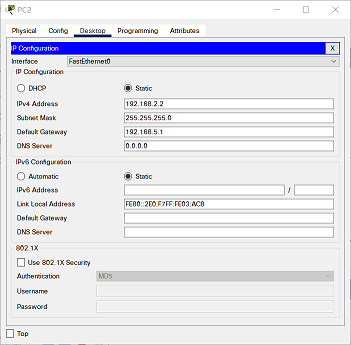
\includegraphics[width=6cm]{PC2.png}
        \caption{PC2配置}
    \end{minipage}
    \begin{minipage}[t]{0.48\textwidth}
        \centering
        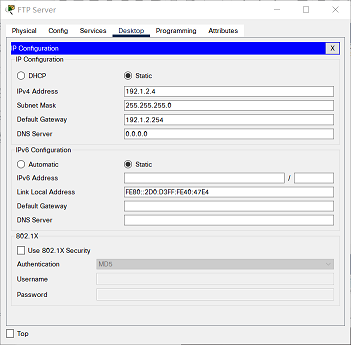
\includegraphics[width=6cm]{FTP服务器配置.png}
        \caption{FTP服务器配置}
    \end{minipage}
\end{figure}

\begin{figure}[h]
    \centering
    \begin{minipage}[t]{0.48\textwidth}
        \centering
        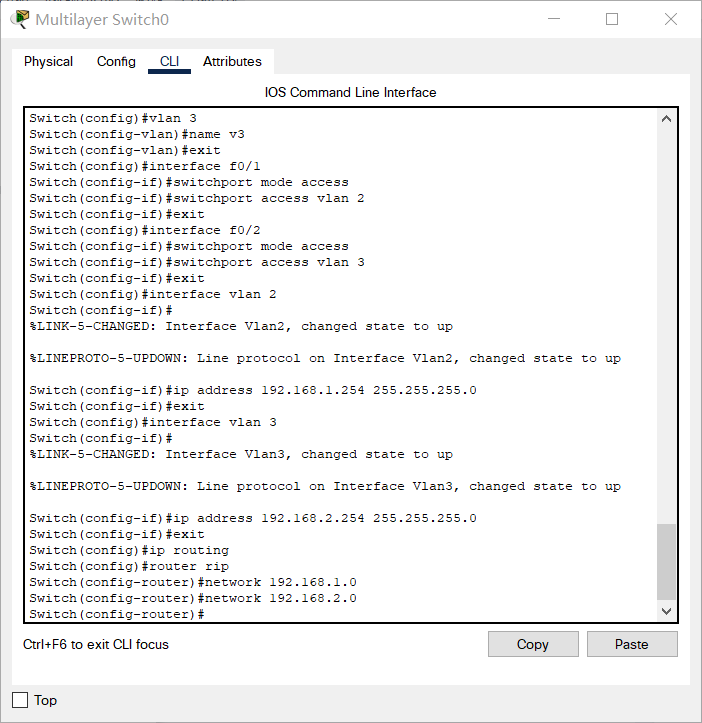
\includegraphics[width=6cm]{三层交换机1.png}
        \caption{三层交换机配置(1)}
    \end{minipage}
    \begin{minipage}[t]{0.48\textwidth}
        \centering
        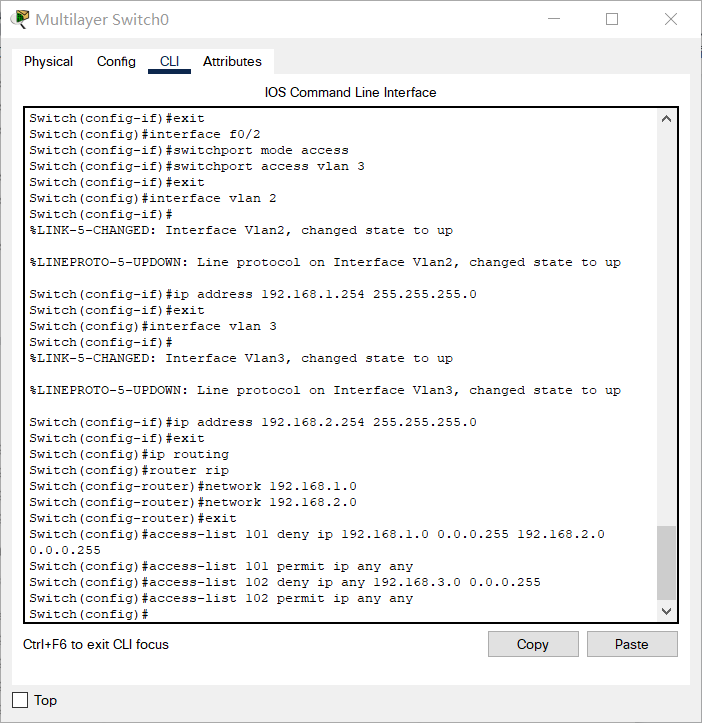
\includegraphics[width=6cm]{三层交换机2.png}
        \caption{三层交换机配置(2)}
    \end{minipage}
\end{figure}

\newpage
\subsubsection{实验结果}
将Admin分别与PC4和PC6进行通信
\begin{figure}[h]
    \centering
    \begin{minipage}[t]{0.48\textwidth}
        \centering
        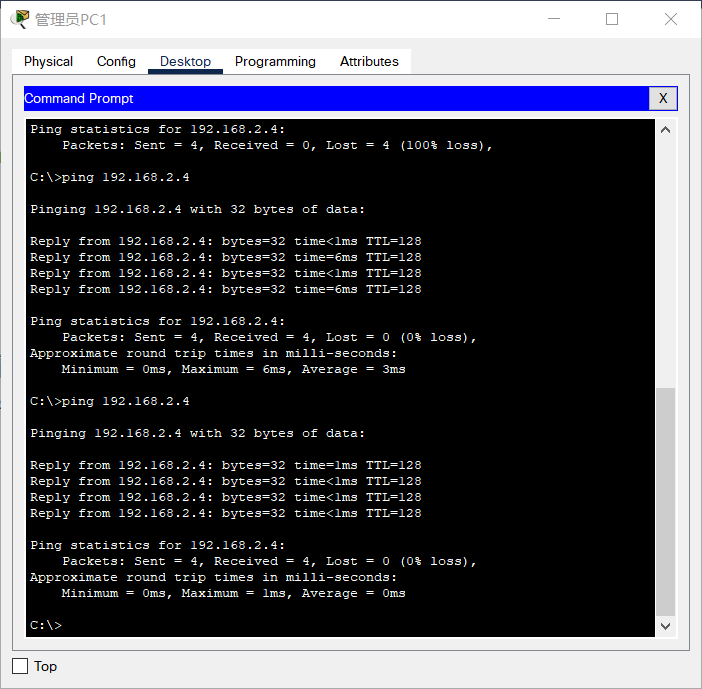
\includegraphics[width=6cm]{PC4.png}
        \caption{Admin与PC4进行通信}
    \end{minipage}
    \begin{minipage}[t]{0.48\textwidth}
        \centering
        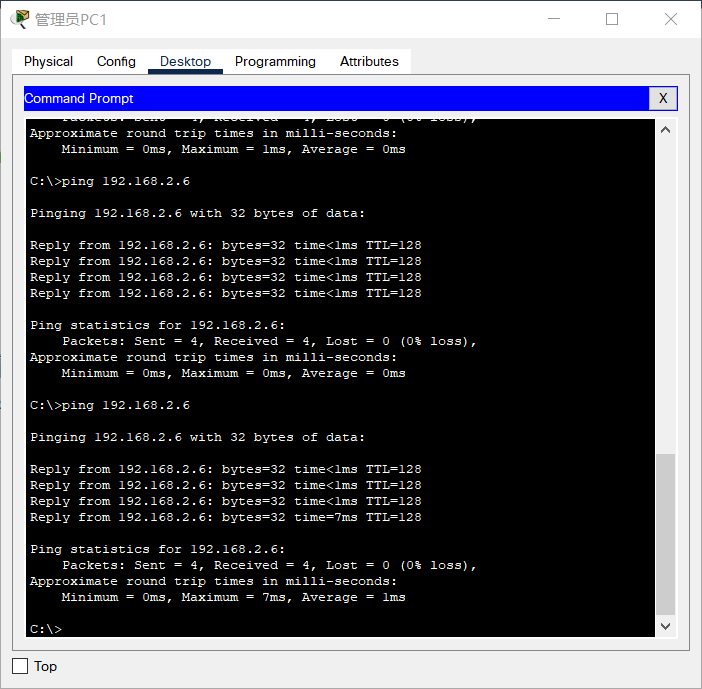
\includegraphics[width=6cm]{PC6.png}
        \caption{Admin与PC6进行通信}
    \end{minipage}
\end{figure}

Admin分别访问ATP服务器和Web服务器

\begin{figure}[h]
    \centering
    \begin{minipage}[t]{0.48\textwidth}
        \centering
        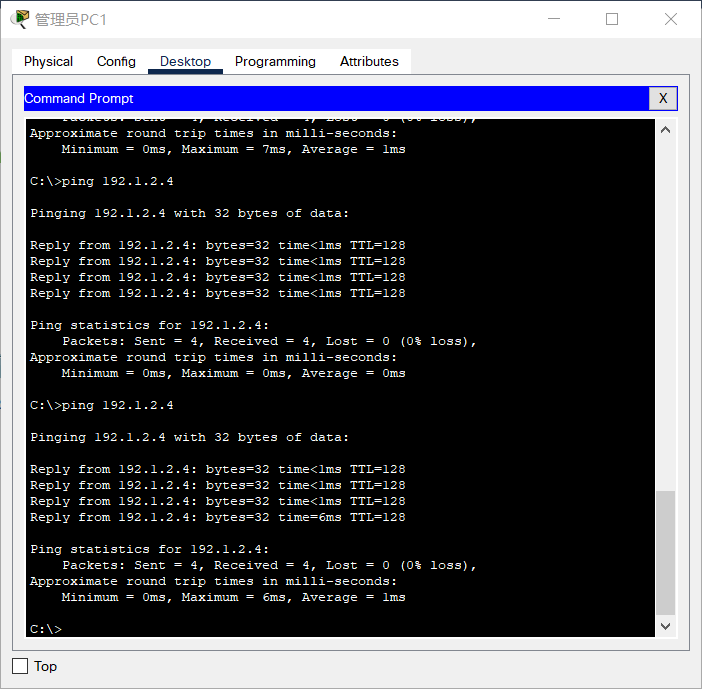
\includegraphics[width=6cm]{ATP.png}
        \caption{Admin访问ATP服务器}
    \end{minipage}
    \begin{minipage}[t]{0.48\textwidth}
        \centering
        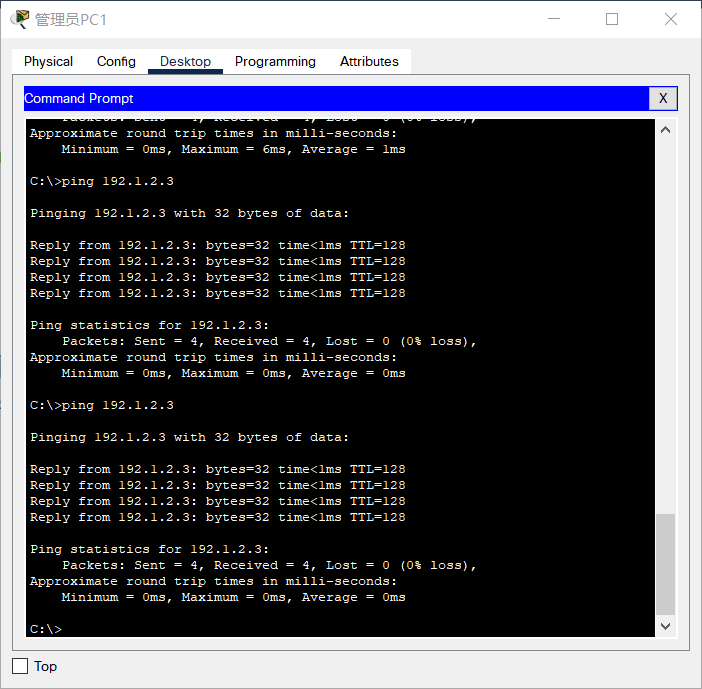
\includegraphics[width=6cm]{wEB.png}
        \caption{Admin访问Web服务器}
    \end{minipage}
\end{figure}
\section{总结与反思}
实验室虚拟化是现在以及今后的一个未来趋势,当虚拟化发展到一定程度后,元宇宙就成为了主流,元宇宙实验室可以做到将真实的实验室搬到每个人的大脑中,实现信息的交互,能够极大地提高教学质量和教学水平。

小组成员心得体会:
\begin{figure}[h]
    \centering
        \centering
        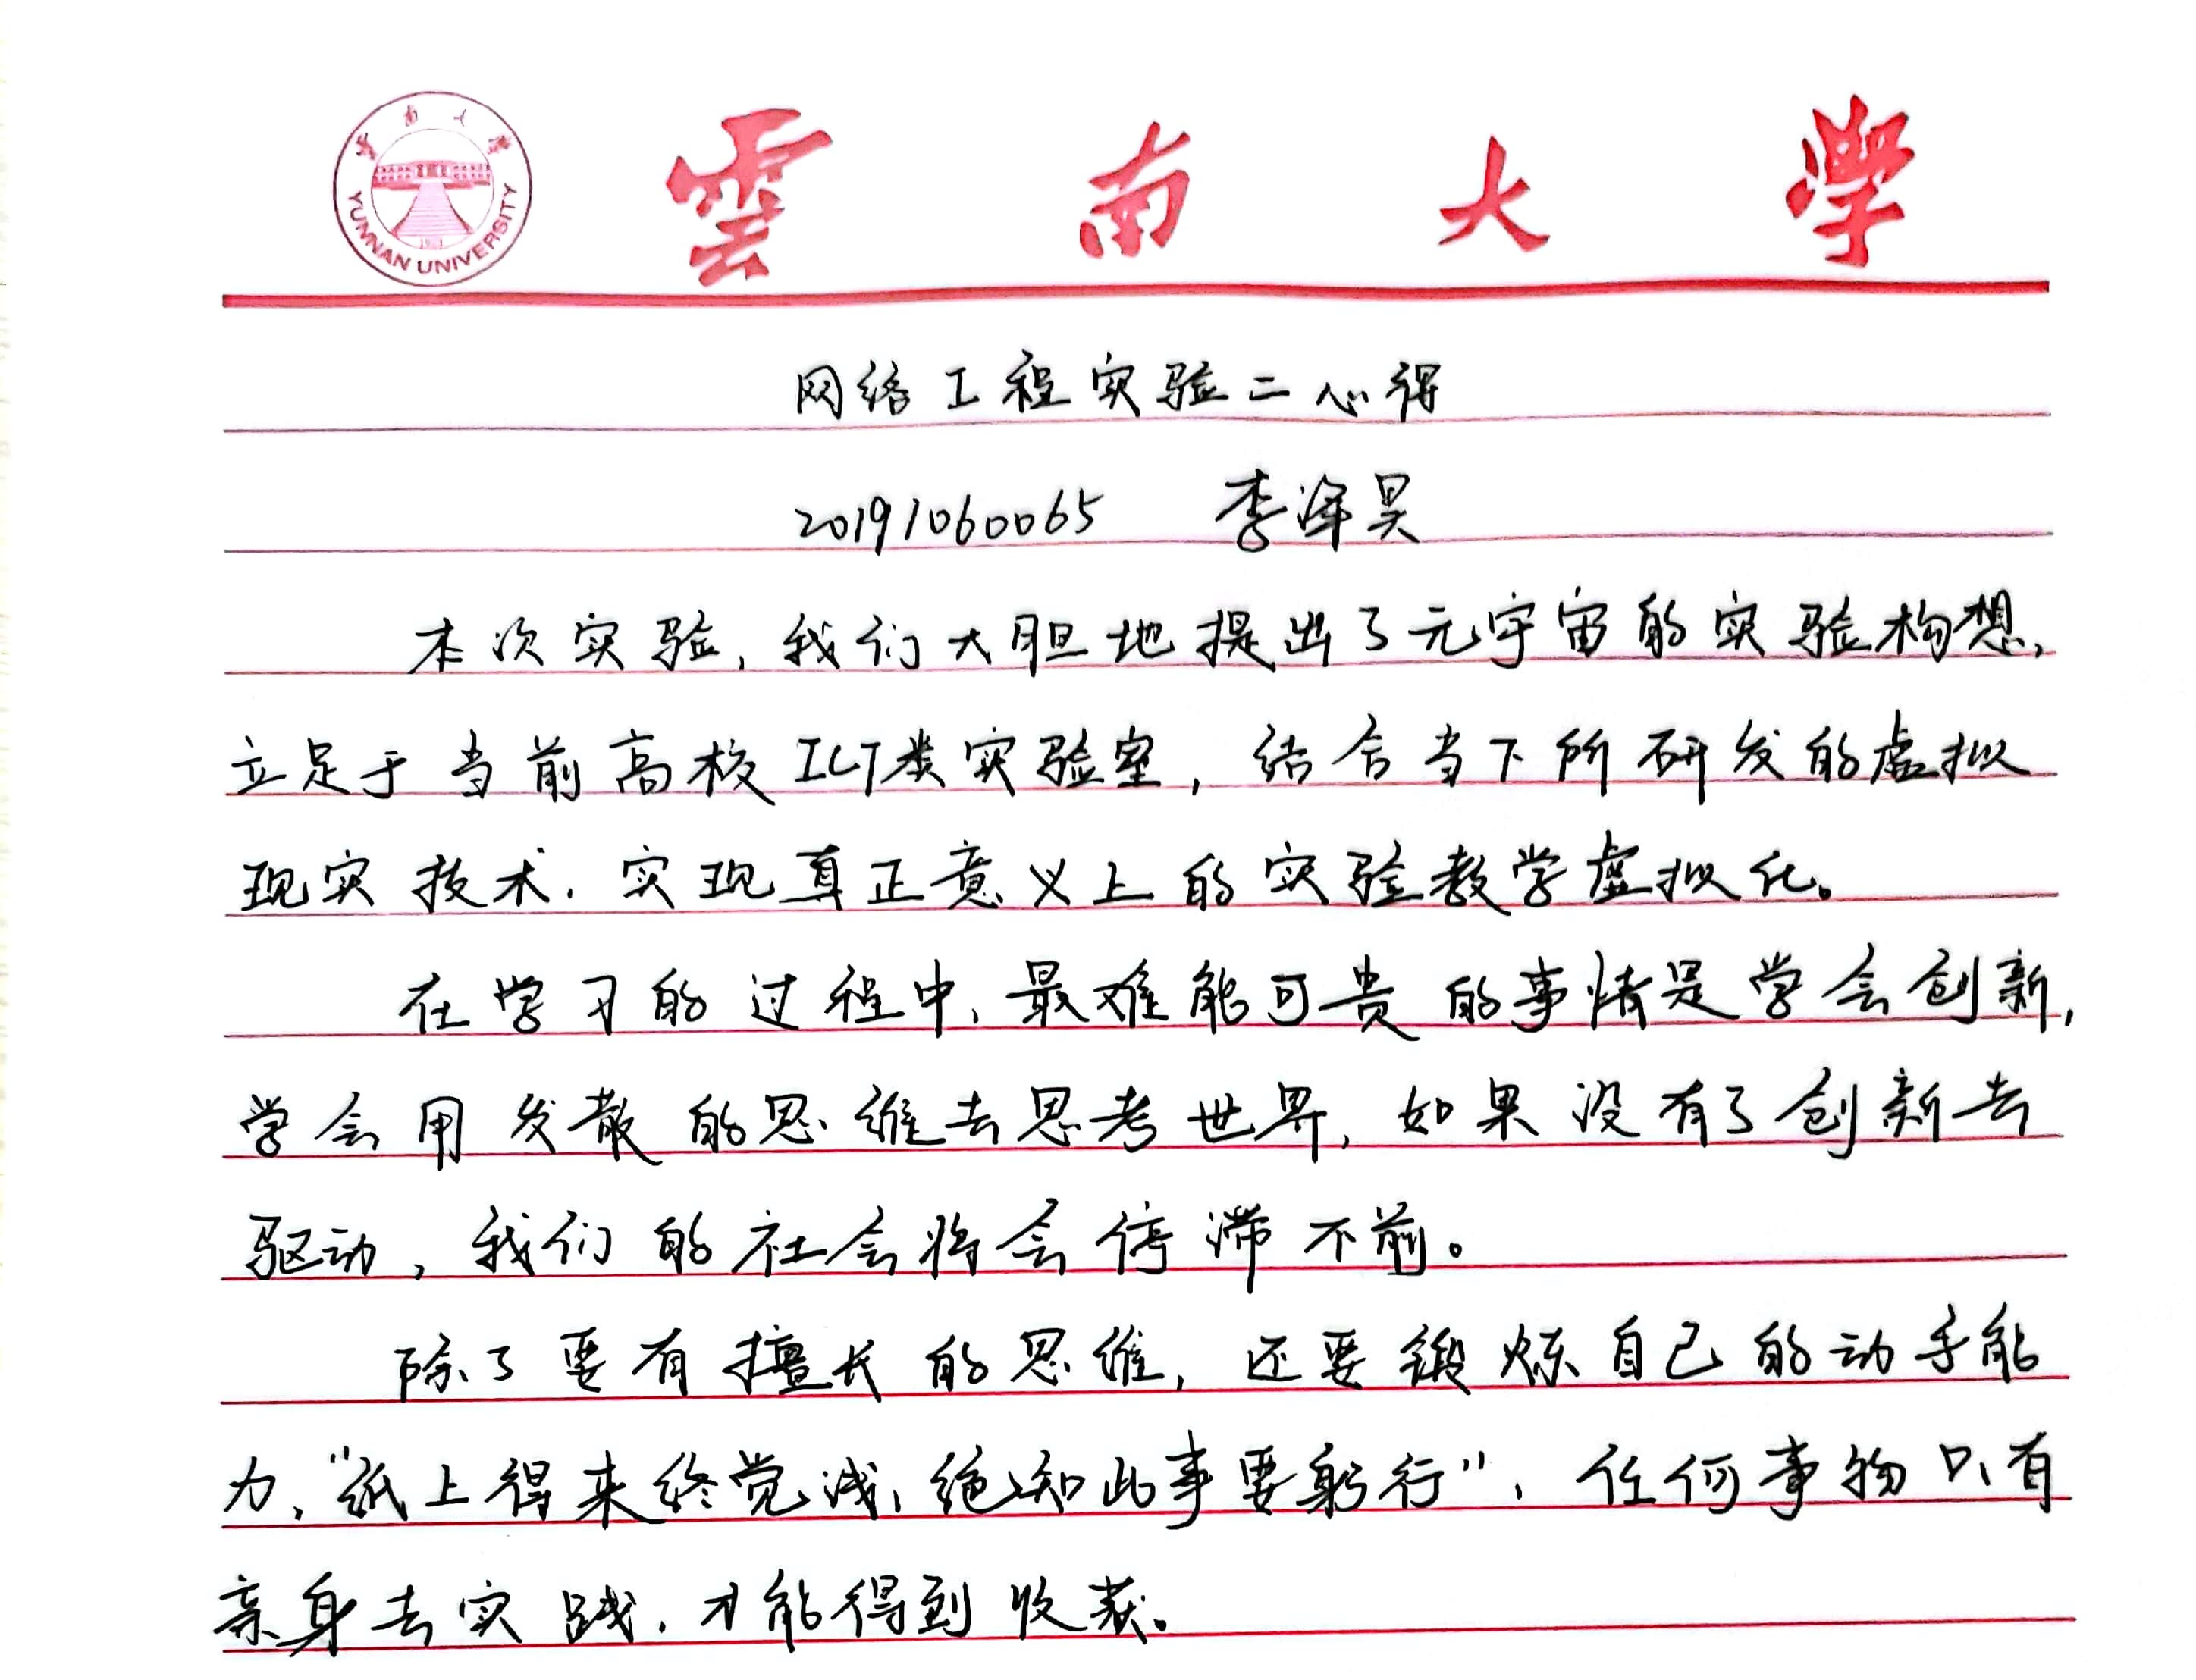
\includegraphics[width=15cm]{lzh.jpg}
        \caption{李泽昊心得体会}
\end{figure}
\begin{figure}[h]
    \centering
        \centering
        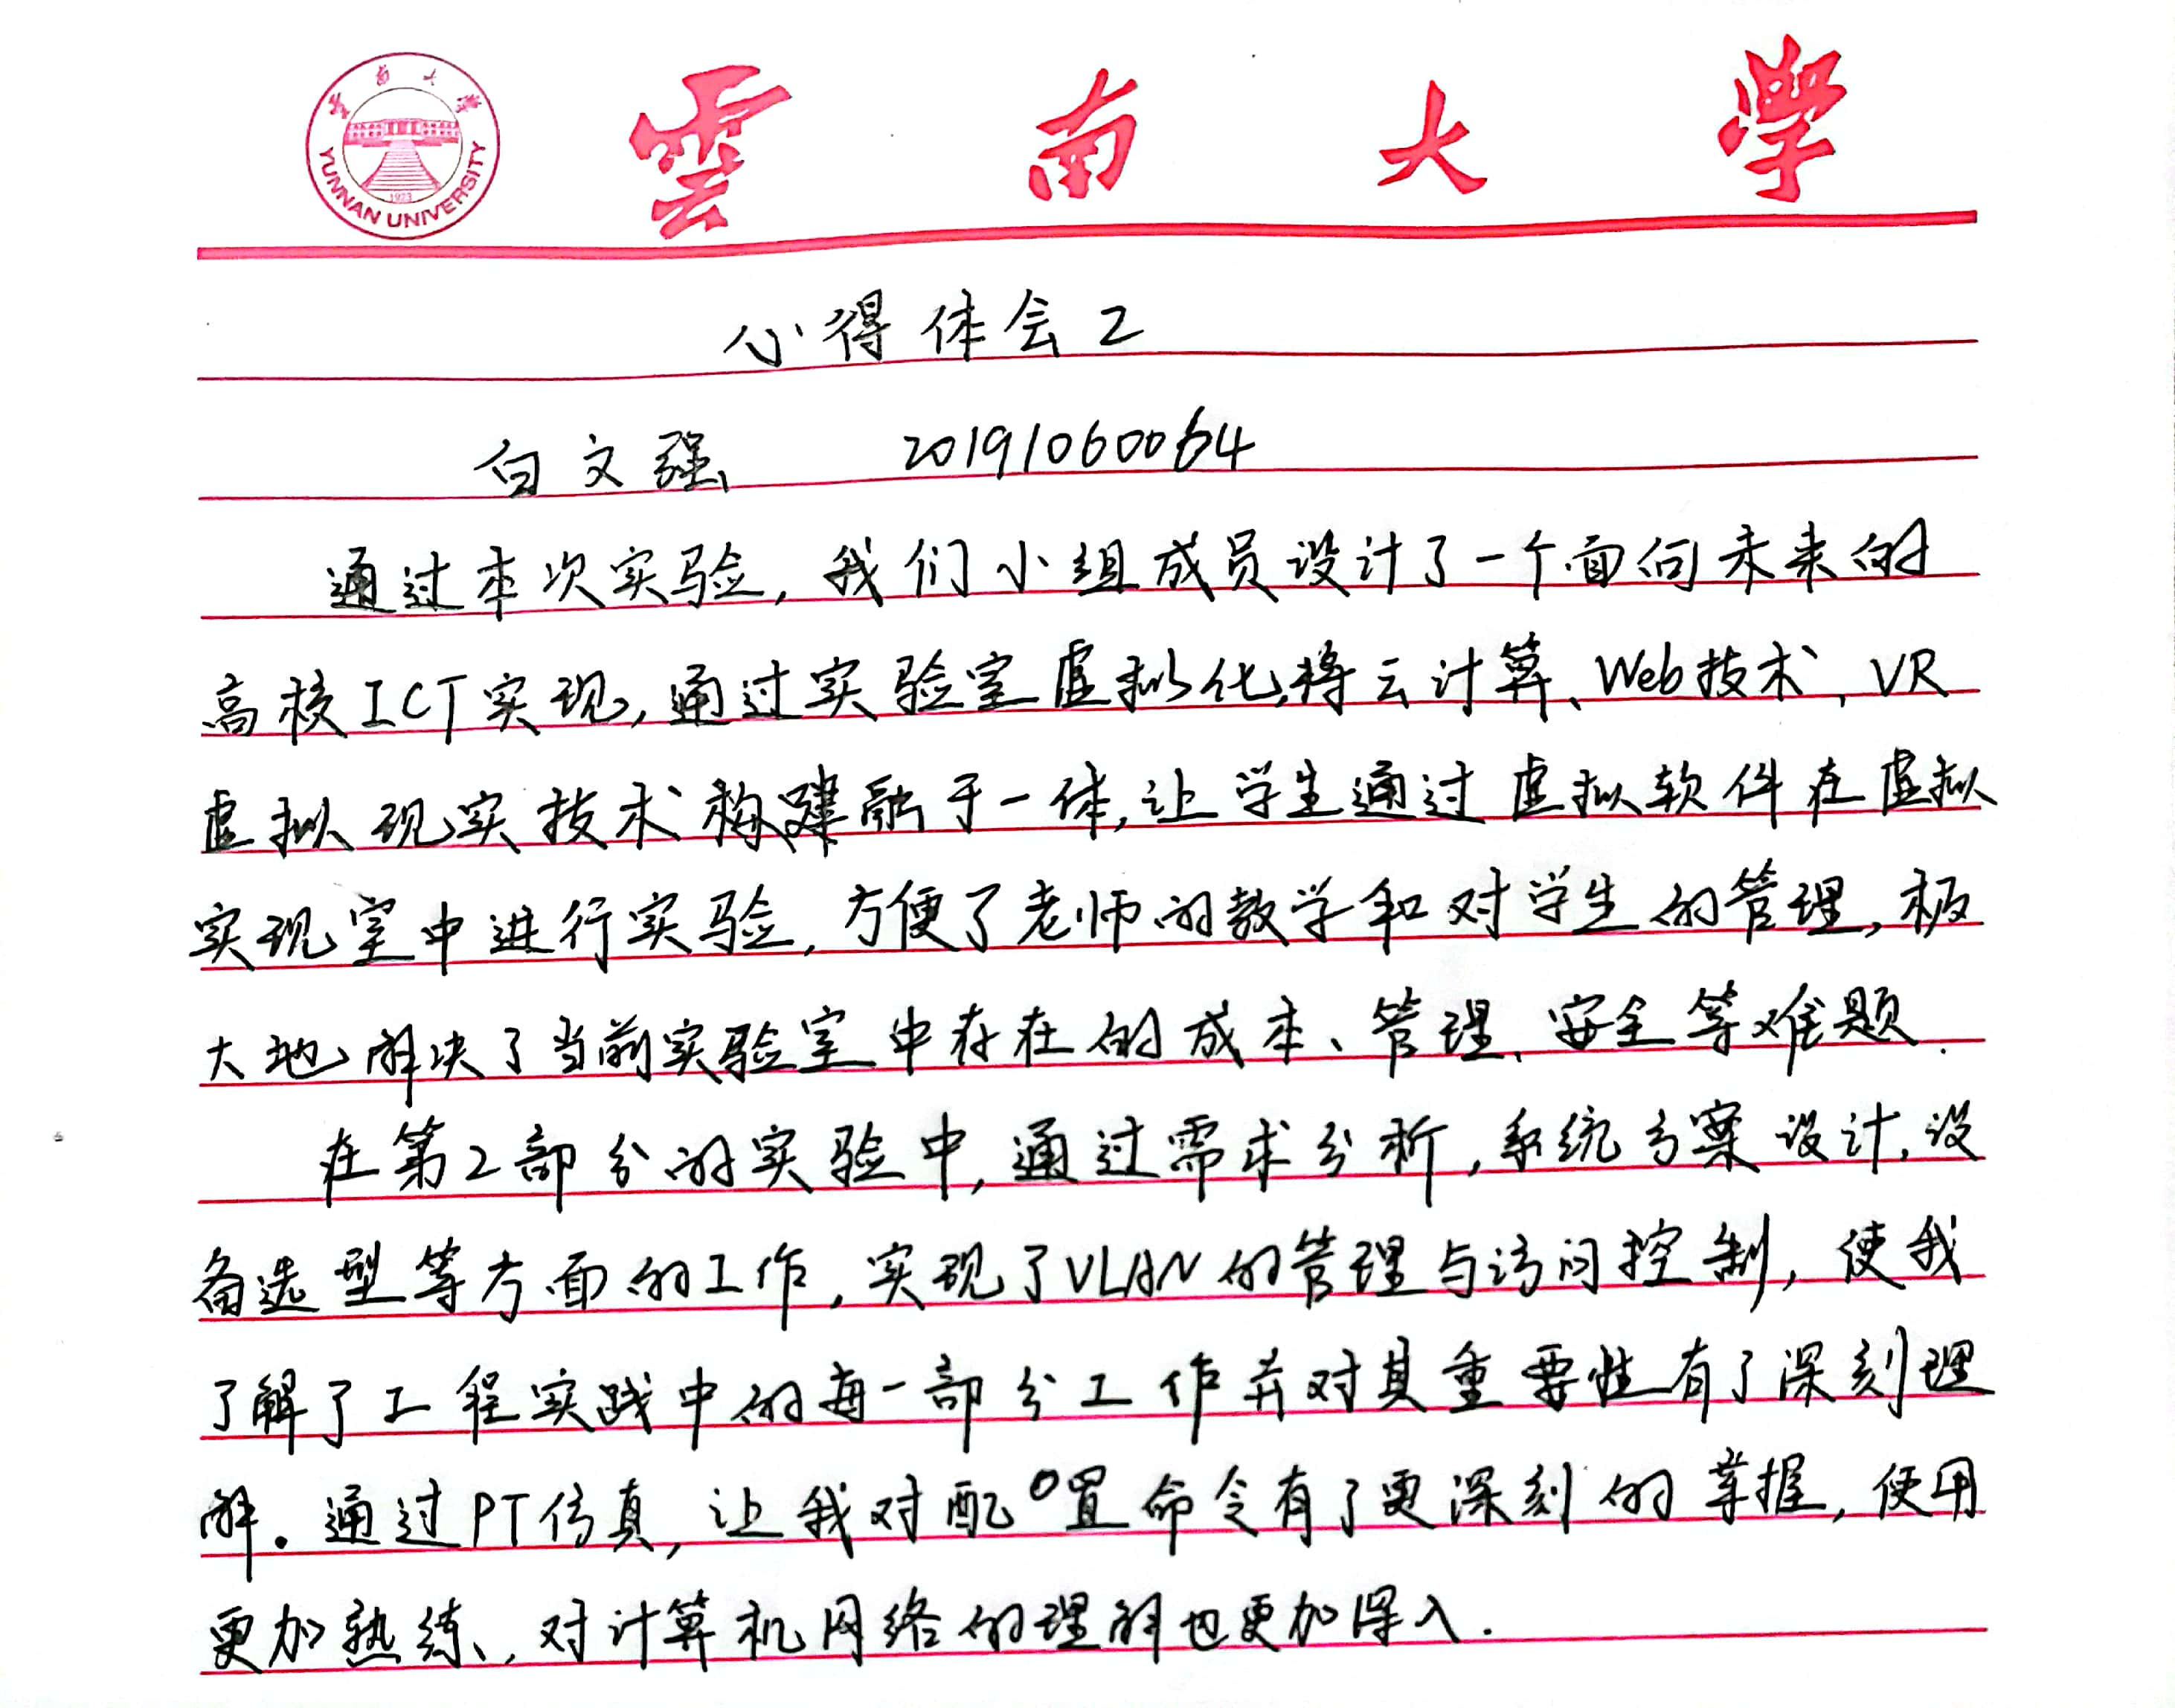
\includegraphics[width=15cm]{bwq.jpg}
        \caption{白文强心得体会}
\end{figure}

\begin{figure}[h]
    \centering
        \centering
        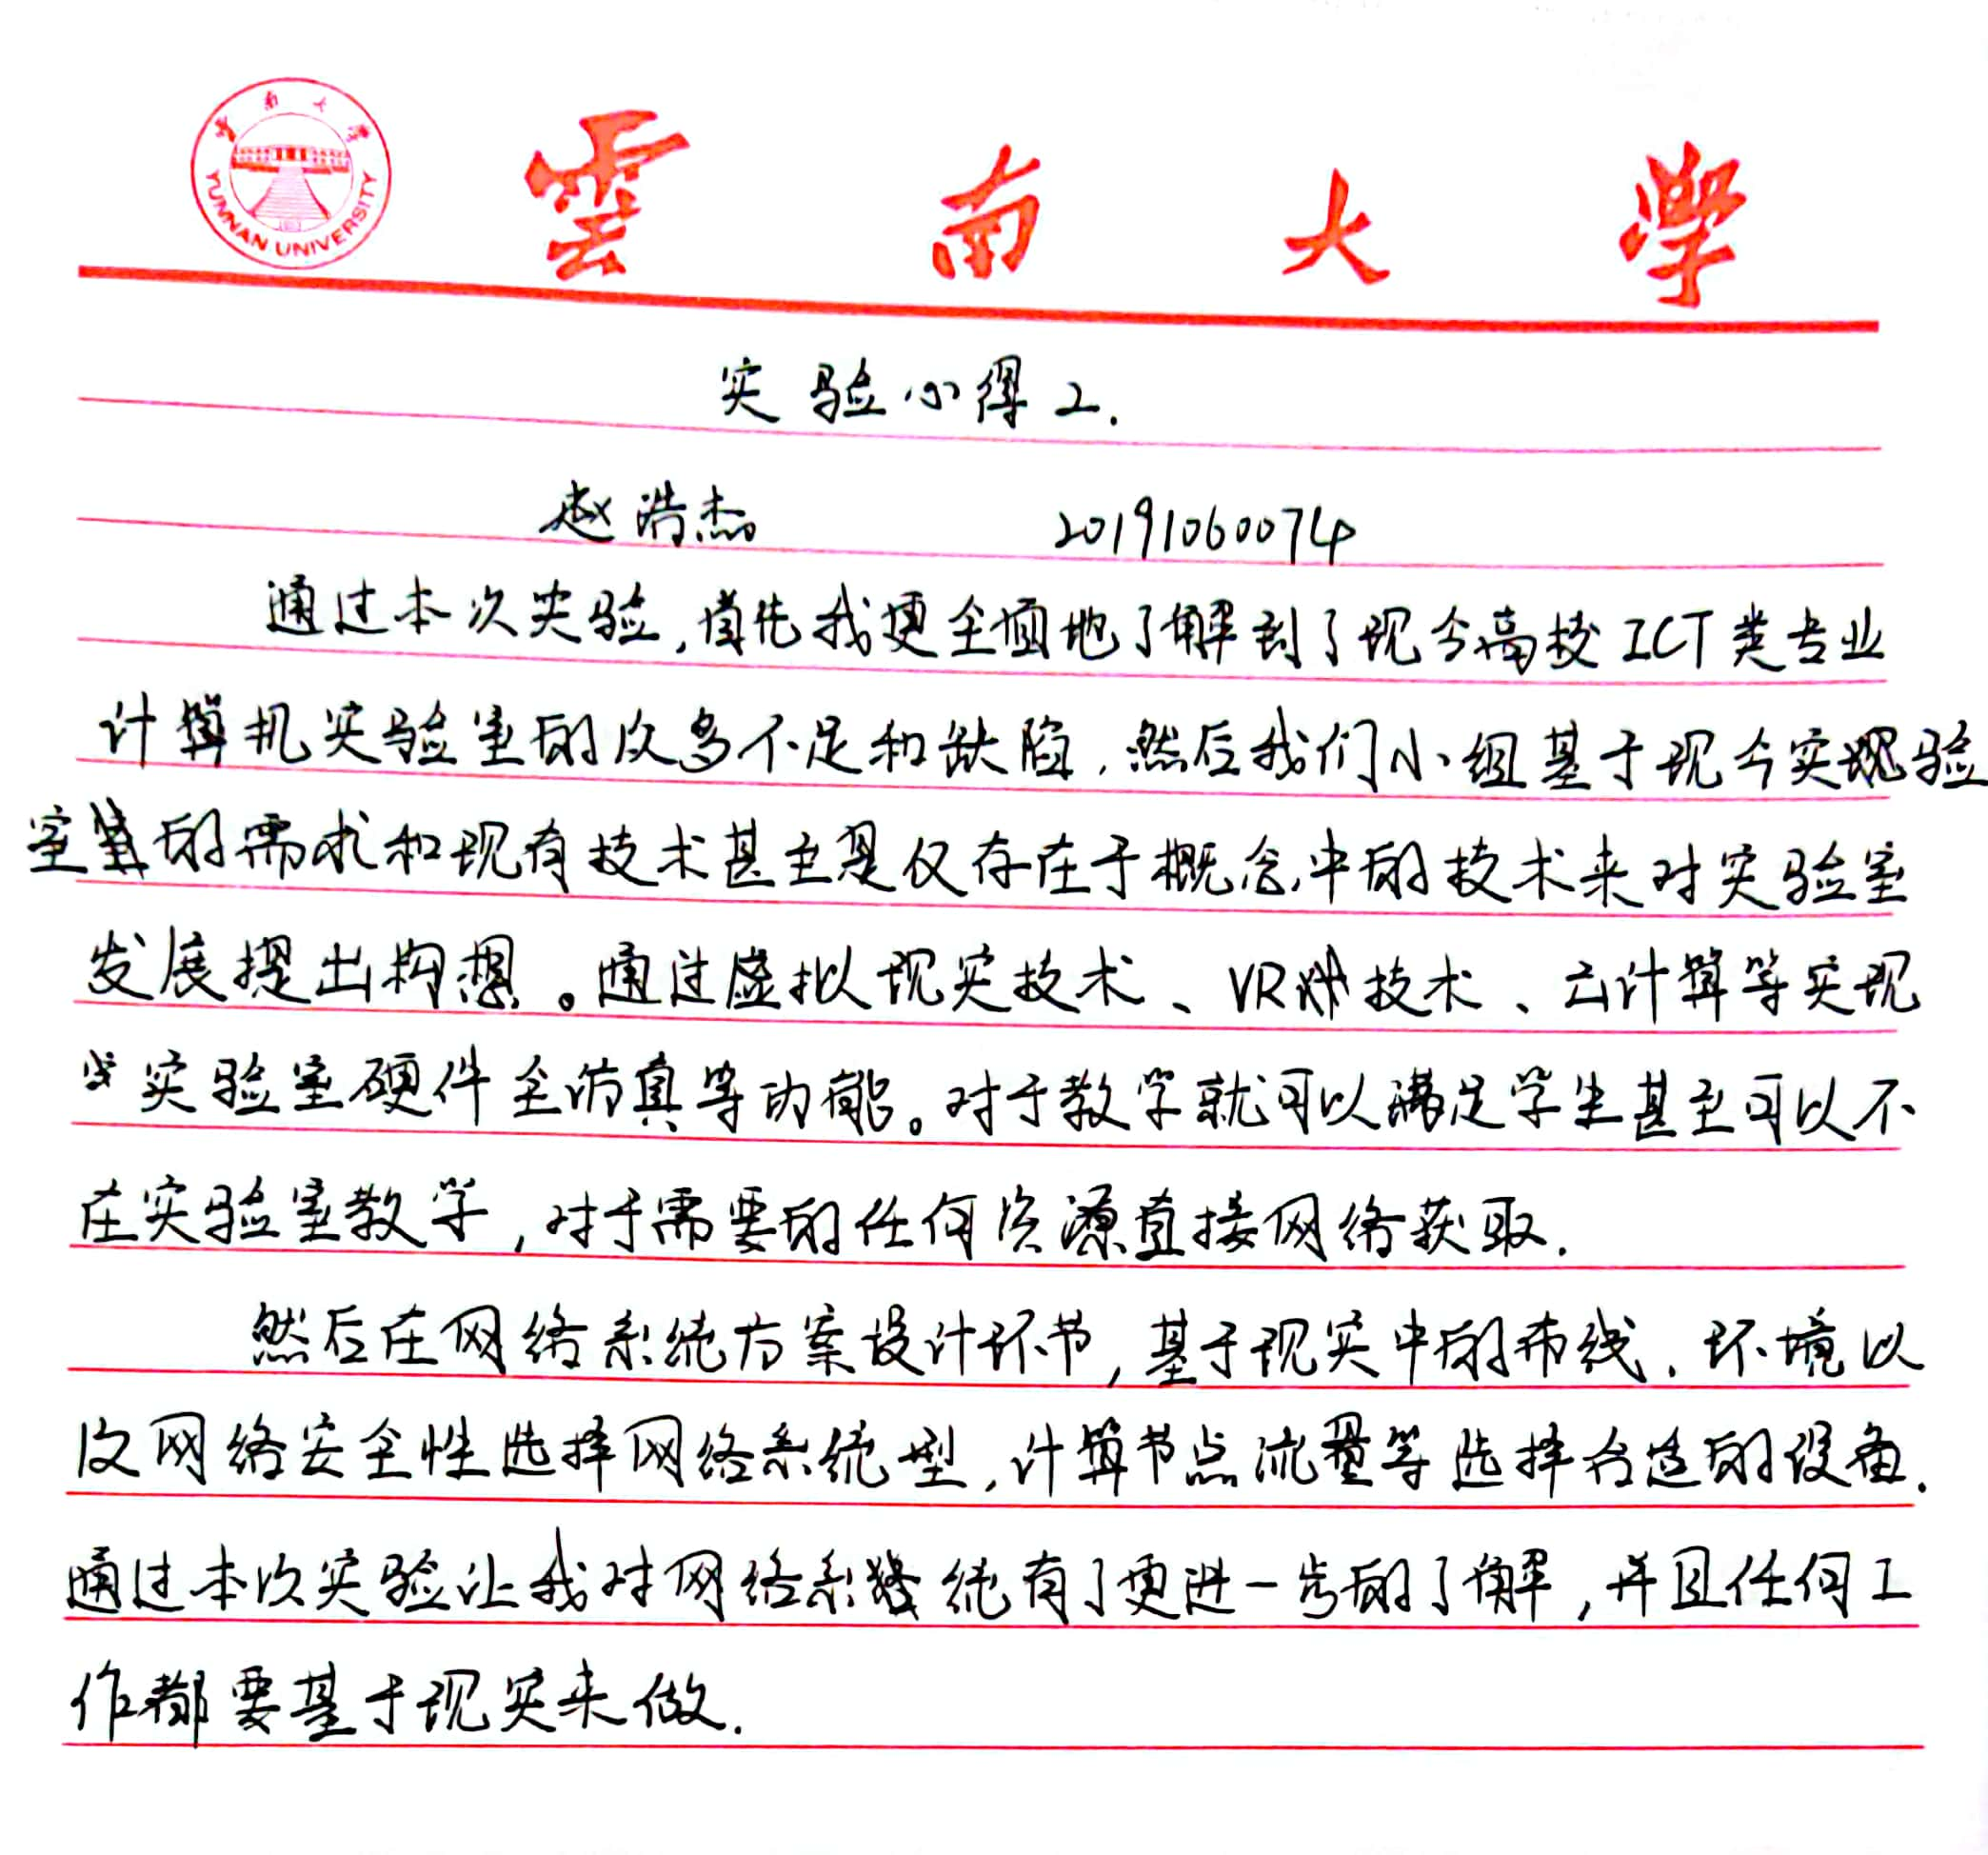
\includegraphics[width=15cm]{赵浩杰.jpg}
        \caption{赵浩杰心得体会}
\end{figure}

\begin{figure}[h]
    \centering
        \centering
        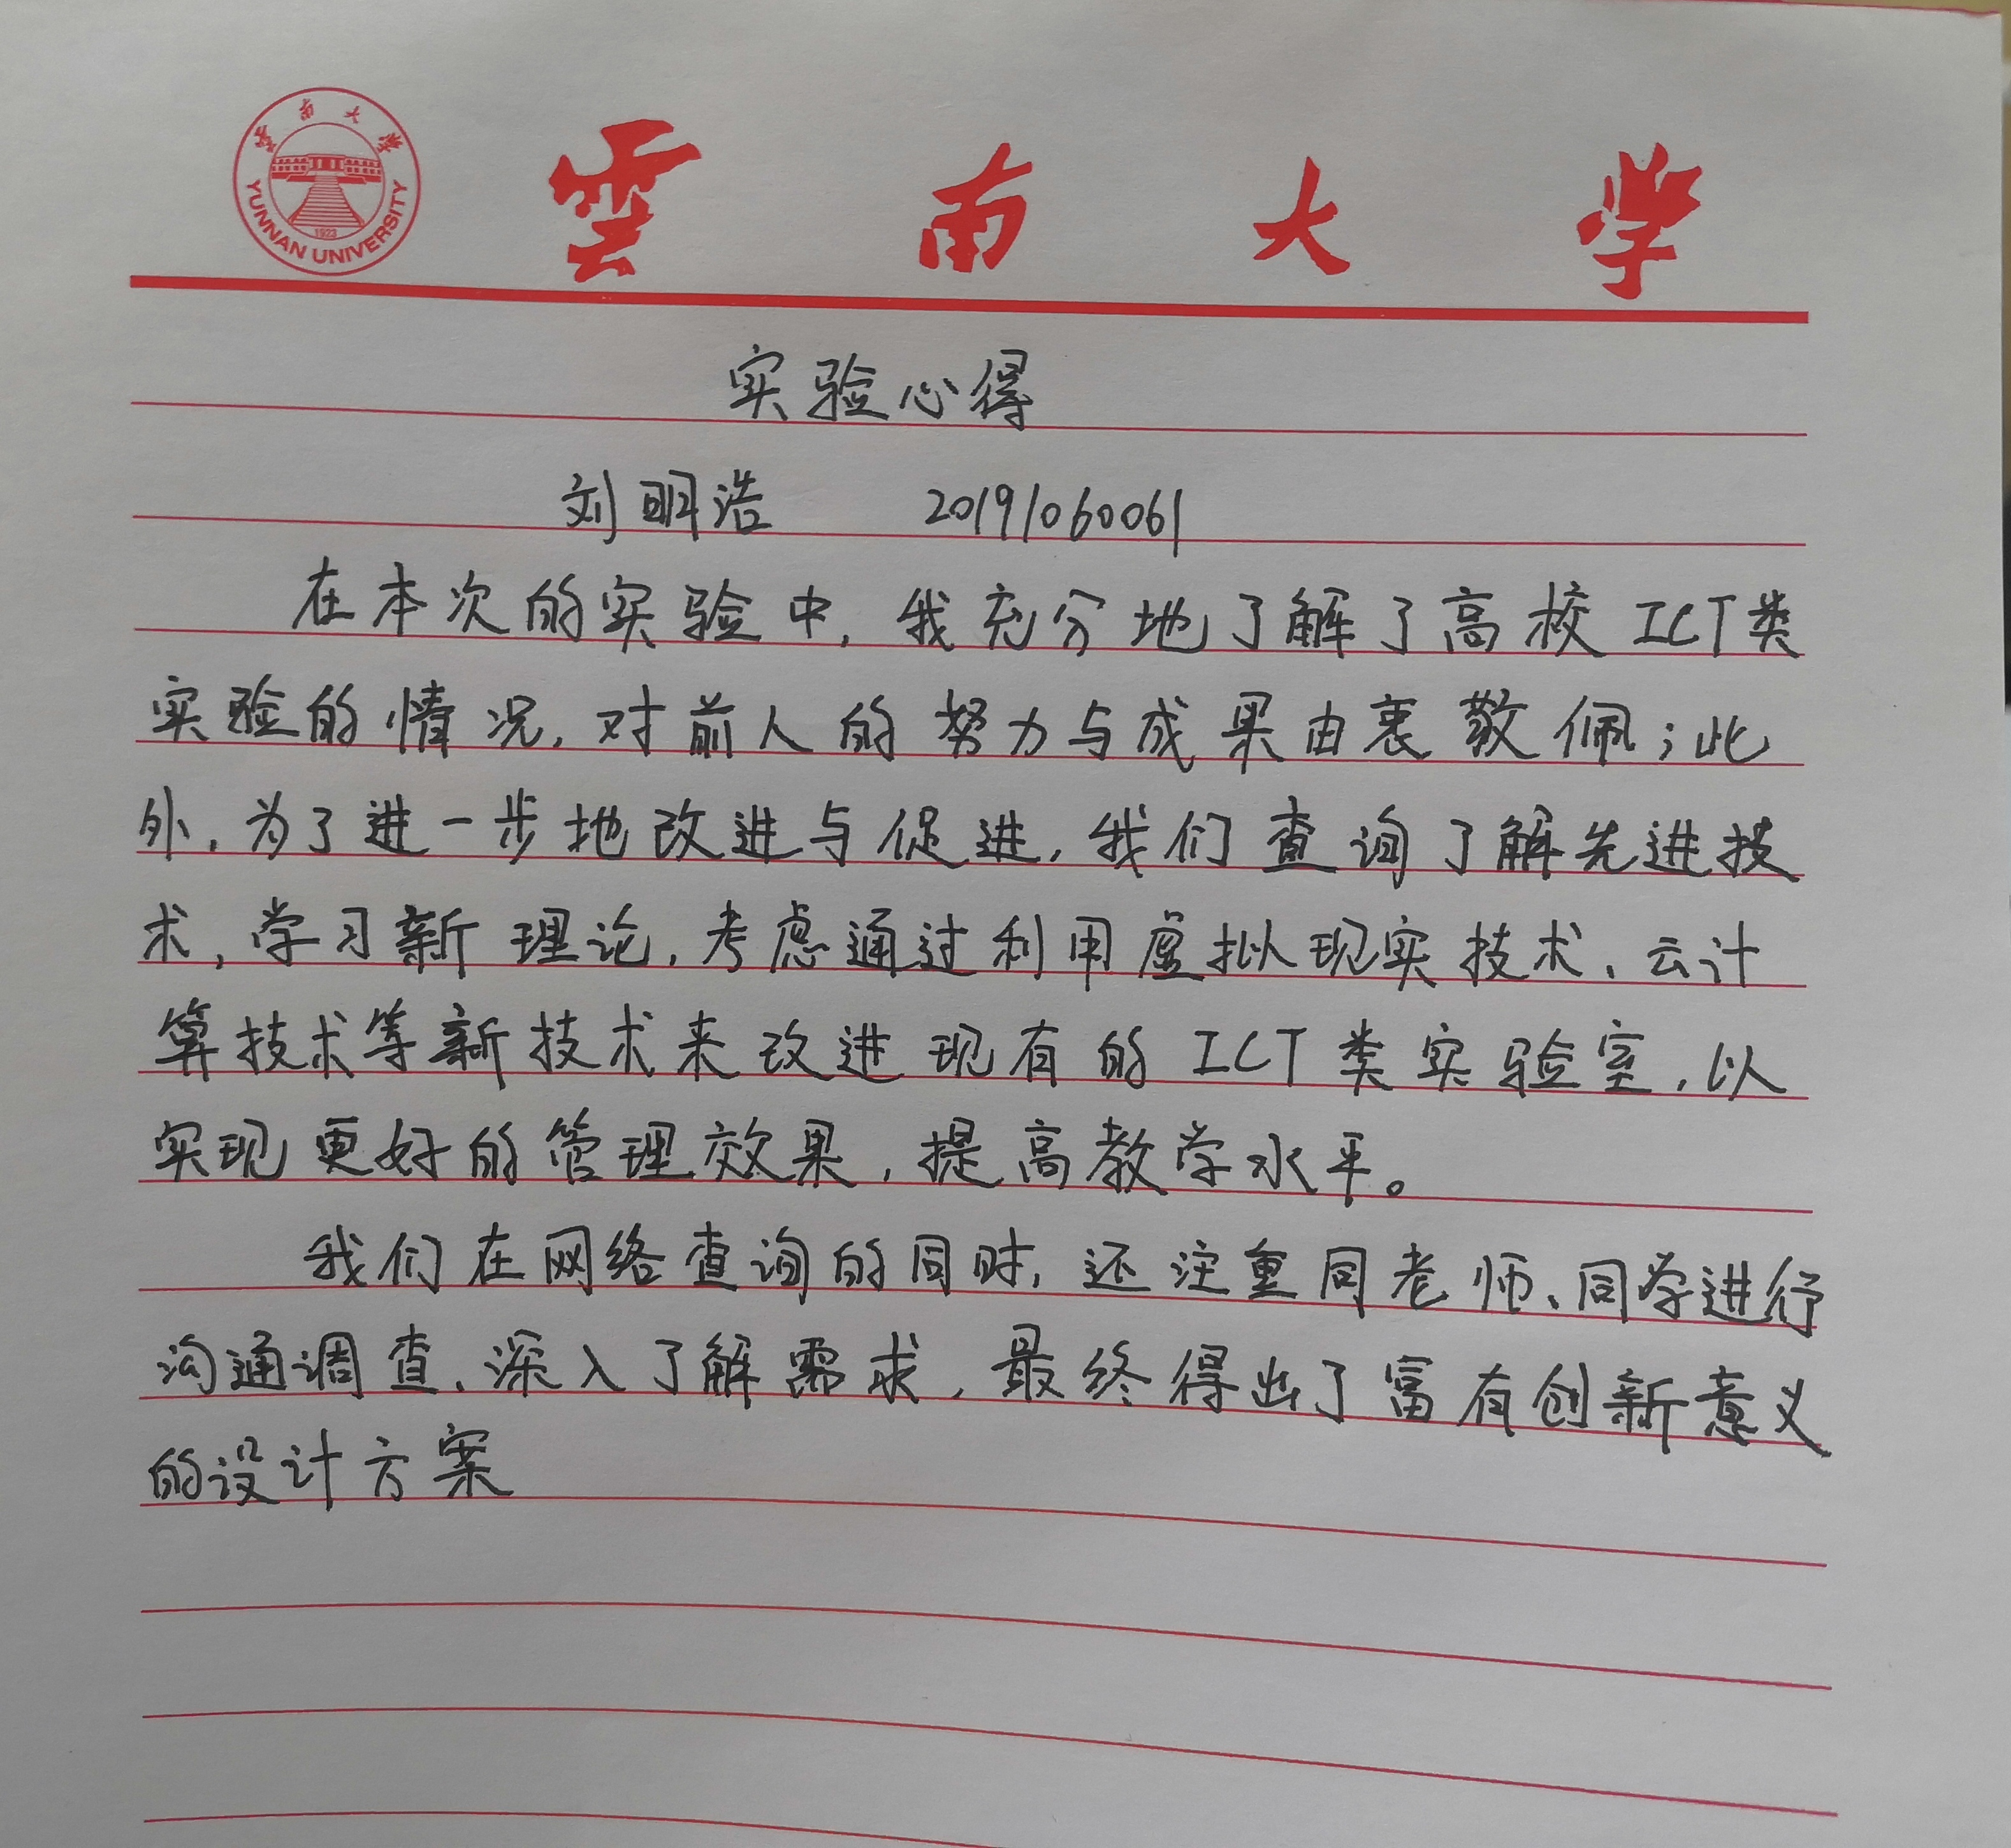
\includegraphics[width=15cm]{lmh.jpg}
        \caption{刘明浩心得体会}
\end{figure}


\begin{figure}[h]
    \centering
        \centering
        
\includegraphics[width=15cm]{yy.jpg}
        \caption{依阳心得体会}
\end{figure}

\newpage
\begin{figure}[h]
    \centering
        \centering
        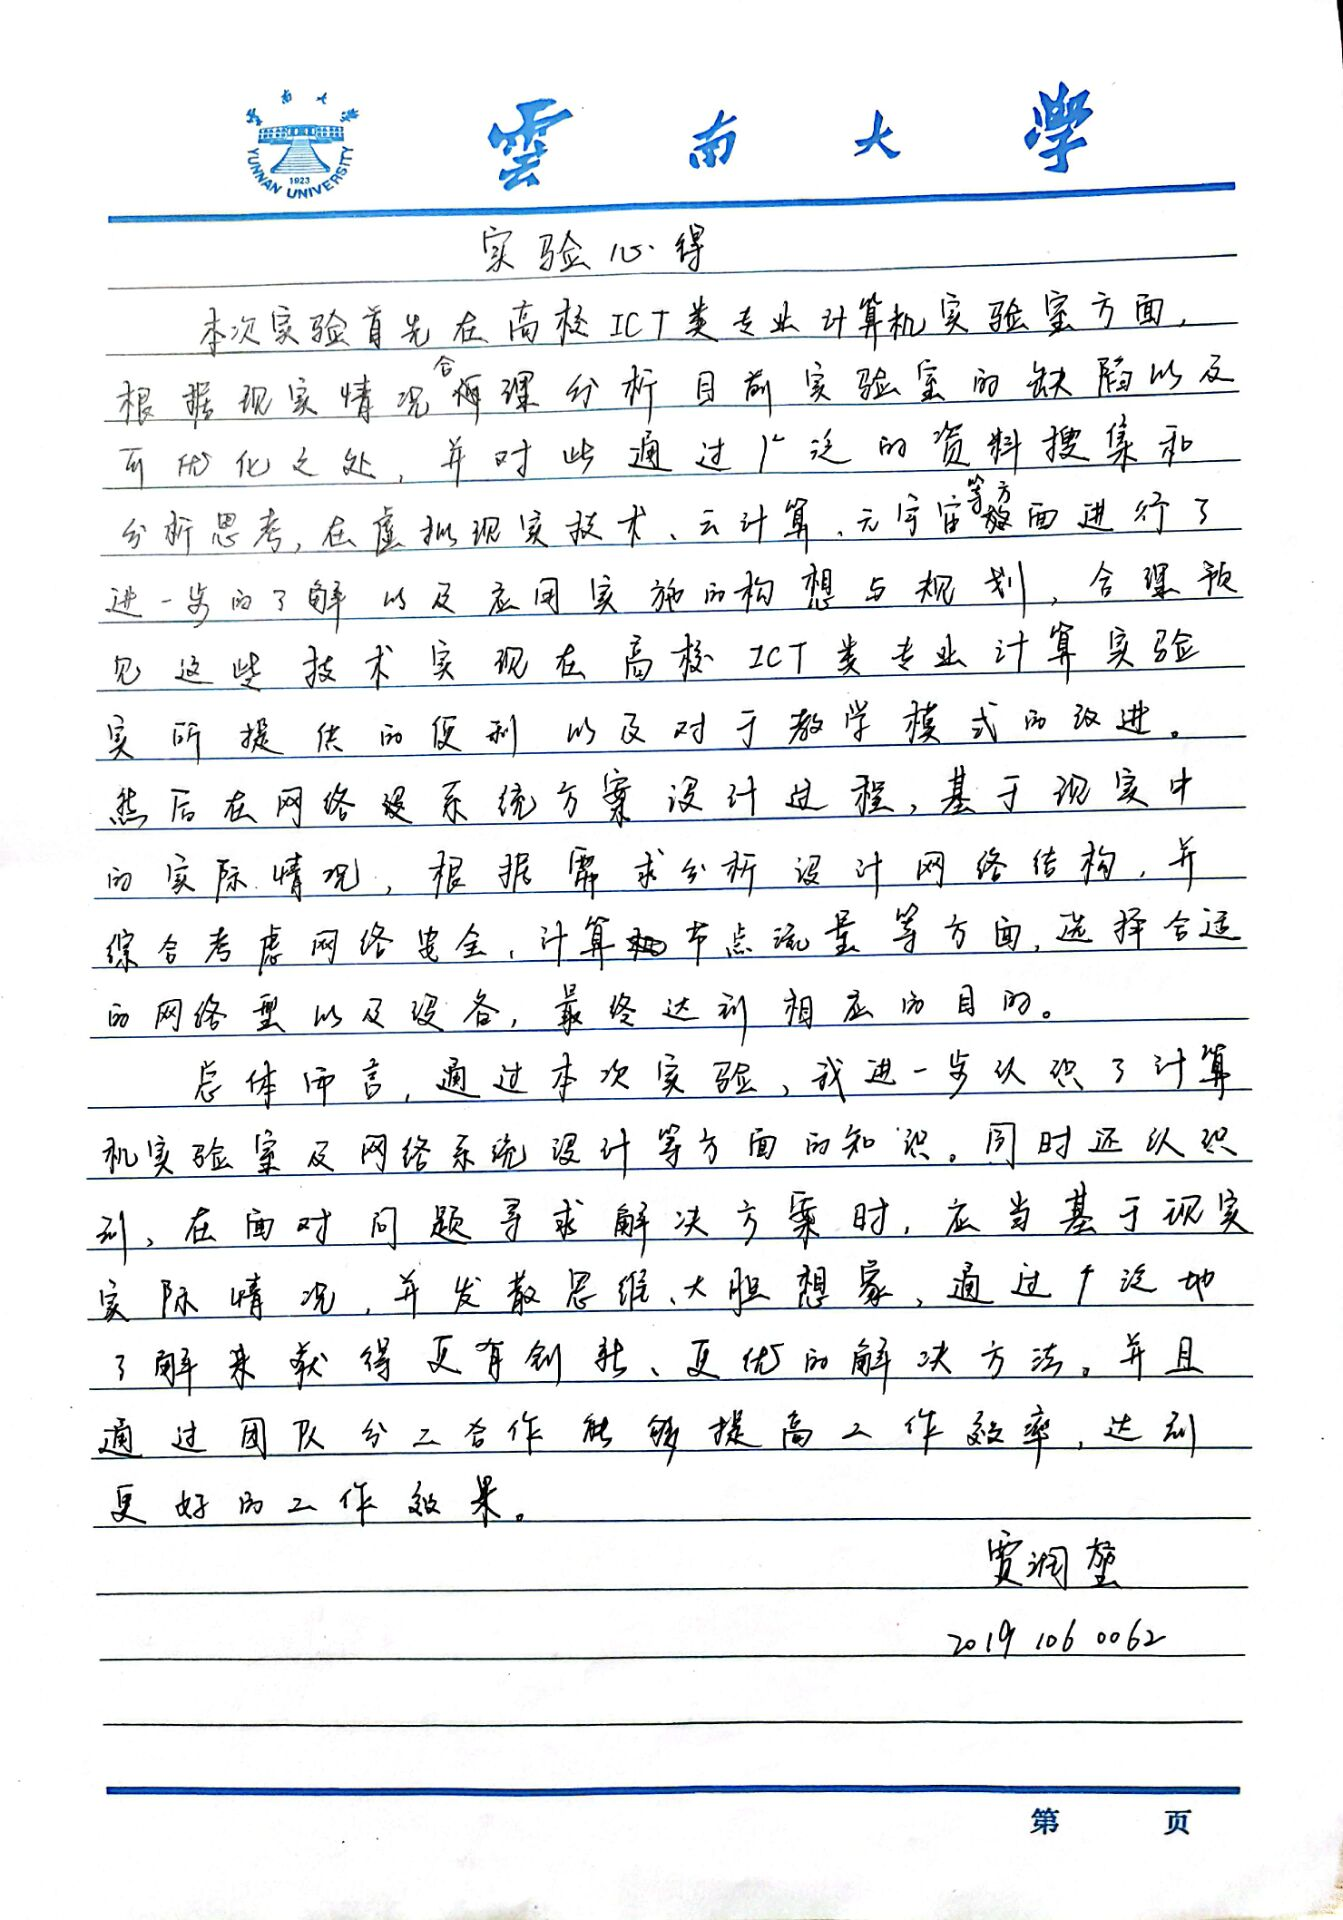
\includegraphics[width=15cm]{hi.jpg}
        \caption{\CJKfontspec{黑体}{贾润堃心得体会}}
\end{figure}

\begin{thebibliography}{1}%个数99  最大为99
\addcontentsline{toc}{section}{参考文献}   %%把参考文献加入目录

\bibitem{ref1}肖艳鹏. 厘清责任边界,破解高校实验室安全管理难题[N]. 中国应急管理报,2021-11-30(003).DOI:10.28046/n.cnki.ncaqs.2021.004127.
\bibitem{ref2}邓朝晖.计算机虚拟实验室的建设与管理研究[J].计算机产品与流通,2020(01):123.
\bibitem{ref3}朱政. AV、VR实体动态捕捉设备及系统[P]. 广东省:CN113377195A,2021-09-10.
\bibitem{ref4}夏蒙.在元宇宙里能干点啥[J].意林,2022(02):9.
\bibitem{ref5}徐尚青,曾大军.高校计算机实验室网络规划及几点问题的思考[J].计算机光盘软件与应用,2014,17(13):231+233.
\end{thebibliography}

\end{document}